\documentclass[11pt]{beamer}
\usetheme{AnnArbor}
\usecolortheme{fly}
\usepackage[utf8]{inputenc}
\usepackage[portuguese]{babel}
\usepackage[T1]{fontenc}
\usepackage{amsmath}
\usepackage{amsfonts}
\usepackage{amssymb}
\usepackage{graphicx}
\usepackage{booktabs}
\usepackage{hyperref}
\author[Miguel Nunes (fc56338)]{Miguel Figueiredo Carmona Simões Nunes\\fc56338\\fc56338@alunos.fc.ul.pt}
\title[Seguros de Saúde]{Seguros de Saúde\\Produção de Documentos Técnicos}
\institute[LEI/TP19]{Licenciatura em Engenharia Informática\\TP19}
\date{}
\begin{document}
\begin{frame}
\titlepage
\end{frame}
\begin{frame}{Tabela de Preços}
\begin{table}[htbp]
  \centering
  \resizebox{!}{3.5cm}{
    \begin{tabular}{|c|c|c|c|}
    \toprule
    Nº Atos Médicos Anuais & Seguro A & Seguro B & Seguro C \\
    \midrule
    10    & 33    & 38    & 56 \\
    \midrule
    20    & 33    & 47,5  & 91 \\
    \midrule
    30    & 39    & 66,5  & 126 \\
    \midrule
    40    & 51    & 85,5  & 161 \\
    \midrule
    50    & 63    & 104,5 & 196 \\
    \midrule
    60    & 75    & 123,5 & 231 \\
    \midrule
    70    & 87    & 142,5 & 266 \\
    \midrule
    80    & 99    & 161,5 & 301 \\
    \midrule
    90    & 111   & 180,5 & 336 \\
    \midrule
    100   & 123   & 199,5 & 371 \\
    \midrule
    110   & 135   & 218,5 & 406 \\
    \midrule
    120   & 147   & 237,5 & 441 \\
    \bottomrule
    \end{tabular}}
  \caption{Tabela de preços em função do número de atos médicos}
  \label{tab1}
\end{table}
\end{frame}
\begin{frame}{Gráfico de Preços}
\begin{figure}[h]
\centering
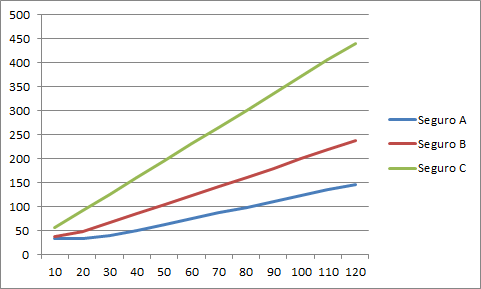
\includegraphics[scale=0.8]{Graph.png}
\caption{Representação gráfica da tabela}
\label{fig1}
\end{figure}
\end{frame}
\begin{frame}{Qual é o melhor seguro?}
O melhor seguro é o seguro A já que, como visto na tabela e no gráfico:
\begin{itemize}
\item A assinatura anual é a mais barata;
\item É o seguro que oferece maior número de atos médicos grátis;
\item É o seguro que depois de finalizados os atos médicos grátis, oferece o melhor preço nos atos médicos seguintes.
\end{itemize}
\end{frame}
\begin{frame}
\begin{figure}[]
\centering

\includegraphics[scale=1]{BeamerSeguro.jpg}
\caption{\href{https://www.jornaldenegocios.pt/mais/analises-deco/detalhe/beneficios-sociais-seguro-de-saude-para-empresas-em-10-licoes}{https://www.jornaldenegocios.pt/mais/analises-deco/detalhe/beneficios-sociais-seguro-de-saude-para-empresas-em-10-licoes}}
\label{fig2}
\end{figure}
\end{frame}
\end{document}
